\exercisetitle{
En el circuito de la figura, usar la carta de Smith para encontrar el SWR de la línea, el coeficiente de reflexión en la carga, la admitancia de carga, la impedancia de entrada de la línea, la distancia desde la carga hasta el primer mínimo de voltaje, y la distancia desde la carga al primer máximo de voltaje.
}
Primero normalizaremos la impedancia en la carga como: $z_l = 1.4 + 0.8j$
\subsection{SWR y $\Gamma$}
Para calcular estos valores usando la carta de smith situamos la impedancia normalizada en la carta y medimos la distancia hasta el origen (0, 0),  usando las diferentes escalas en la parte de abajo podremos obtener los valores.
\begin{figure}[h]
  \centering
  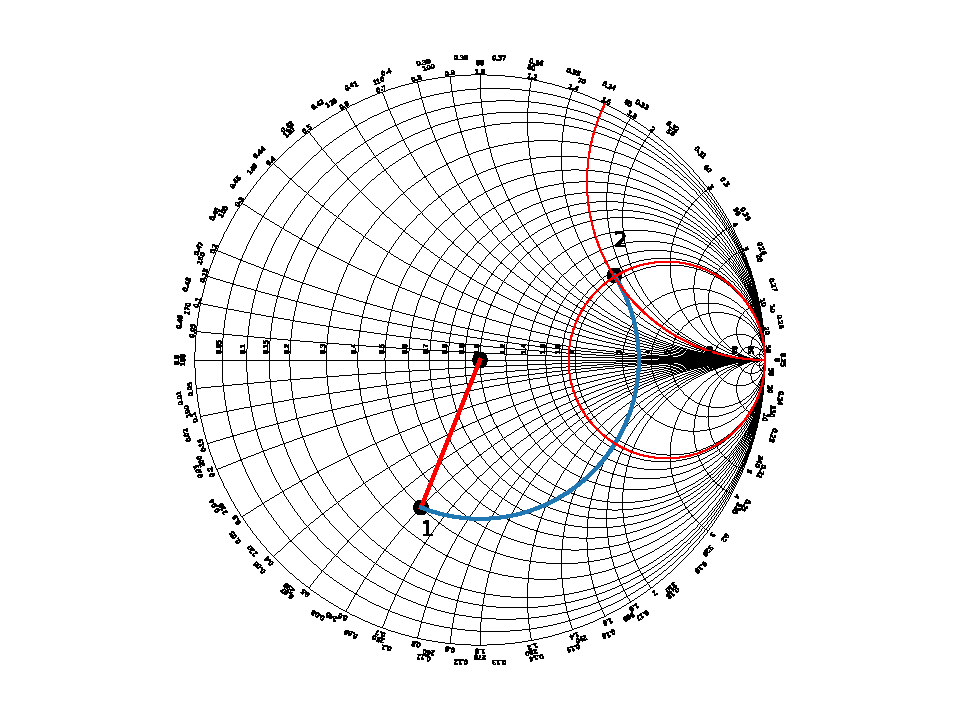
\includegraphics{ej6/images/out2.pdf}
  \caption{Avanzando $0.7\lambda$ hacia la carga}
  \label{ej2smith}
\end{figure}
